\chapter{Implementation}

\section{Introduction}

\subsection{Tools}

As part of this thesis two tools have been developed to gather information about an application:

\texttt{pintool\_static.so} analyses the application and all its shared libraries and creates a database with all the locations in the source code where a tag can be placed. More details are present in Section \ref{cap3:pintoolstatic}.

\texttt{pintool\_dynamic.so} is an Intel Pin tool that performs tracing of the target application. It uses the database created by \texttt{pintool\_static.so} and adds all the gathered information. The tool is extensively explained in Section \ref{cap3:pintooldynamic}.

\subsection{Analyses}

To improve te usefulness of the gathered data some automated analyses have been developed to extract useful insights into applications. Currently two are implemented:

\textbf{Section Analysis} show the potential speedup and dependencies when executing sections of code in parallel to each other.

\textbf{Pipeline Analysis} determines the speedup and dependencies when applying the pipeline parallelization pattern to a loop.

It is also possible to easily add additional analyses to either \texttt{pintool\_dynamic.so} or the database processing.

\subsection{Visualizations}

The database created by \texttt{pintool\_dynamic.so} is compatible with the format used by Parceive, but it adds some additional data. Existing views continue to work and have been extended to display tag information.

Specialized views have been developed to display the information provided by the implemented analyses. Additional views can also be developed due to the use of the generic framework.

\subsection{Workflow}

\begin{figure}
	\centering
	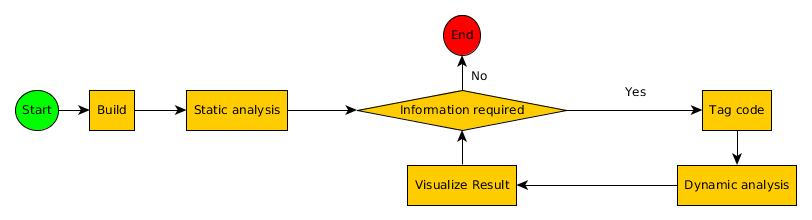
\includegraphics[width=1\textwidth]{workflow}
	\caption{User workflow}
	\label{cap3:workflow}
\end{figure}

Figure \ref{cap3:workflow} shows the workflow when using our tools.  Because we are using dynamic binary instrumentation a user must first build the application executable. The static analysis needs to be executed every time the program is modified and rebuilt.

The dynamic analysis can be executed multiple times to gather more information. First the user tags sections of the source code and runs the analysis. The visualizations provide useful information about the executed program and the user can choose to perform another analysis if more data is required.

\subsection{Architecture}

Figure \ref{architecture} shows the architecture of the entire project. It is similar to the one used by Parceive as shown in Figure \ref{parceive:architecture}, sharing the Node.js server and browser architecture.

\begin{figure}
	\centering
	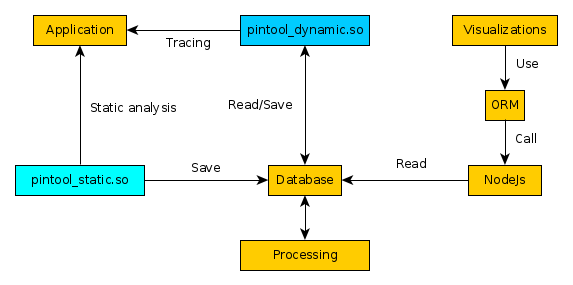
\includegraphics[width=1\textwidth]{architecture}
	\caption{System architecture}
	\label{architecture}
\end{figure}

The split between the dynamic and static analysis was needed because the user must be able to tag the source code of the application before tracing is performed. The database processing, the Node.js server and the ORM have been extended to support our use cases.

\texttt{pintool\_static.so} is responsible for generating the database structure and storing static information about the application. \texttt{pintool\_dynamic.so} uses an existing database to store all the tracing data.

\section{Concepts}

\subsection{Filtering}

By using dynamic binary instrumentation it is possible to process the entire instruction stream of an application, even dynamic libraries and setup code generated by the compiler. Recording all the actions an application performs might be an advantage, but comes at the cost of runtime overhead and a large tracing database. If a developer is not interested in analyzing the entire application the overhead and the size can be reduced by defining parts that should be ignored.

In Parceive and our implementations three types of filters are available:

\textbf{Image} represents the executable or a shared library and can be used to easily ignore code that is not being developed.

\textbf{Function} represents a routine in the executable. This can be used to filter out modules from inside the executable or shared libraries based on the naming convention of the project.

\textbf{File} allows a developer to filter functions based on the file they were defined in. This requires debug for the component that contains the function. This is also the easiest way to only consider code that has debug information.

A very useful example can be see in Figure \ref{cap3:filter-example}. This filter is very practical as it ignores all system libraries, functions without debug information an compiler generated code.

\begin{figure}
	\begin{center}
		\begin{minted}{yaml}
image:
  exclude:
    - /lib64/*
file:
  exclude:
    - /usr/include
    - Unknown
function:
  exclude:
    - _GLOBAL__*
    - __static_initialization_and_destruction_0
		\end{minted}
	\end{center}
	\caption{\texttt{filter.yaml} example}
	\label{cap3:filter-example}
\end{figure}

\subsection{Tagging}

Tags are used to mark interesting parts of the code and to provide input to automatic program analyses. Multiple tag types are currently available:

\textbf{Section} marks the boundaries of a section of code that can be executed in parallel.

\textbf{SectionTask} is a task inside a section. Each task can be run in parallel to any other task.

\textbf{Pipeline} marks the boundaries of a section of code that can be executed in parallel using the pipeline architecture.

\textbf{PipelineIteration} represents one iteration of the pipeline.

\textbf{PipelineSection} is a section of a iteration. These sections can be run in parallel to different sections from different iterations.

\subsubsection{Controling tracing}
\label{controllingtracing}

Filtering can reduce the amount of data gathered during a programs execution, but tags can provide an even more flexible approach. Using tags it is possible to control tracing during execution with the granularity of a line:

\textbf{IgnoreAll} stops all tracing.

\textbf{IgnoreCalls} stops the tracing of calls.

\textbf{IgnoreAccesses} stops the tracing of accesses.

\textbf{ProcessAll} forces the tracing of everything.

\textbf{ProcessCalls} forces the tracing of calls.

\textbf{ProcessAccesses} starts the tracing of accesses.

In Figure \ref{cap3:contralg} we can see the algorithm used to determine whether tracing is performed.

\begin{figure}
	\begin{center}
		\begin{minted}{c}
if (ignoreCalls)
	processCallsComputed = false;
else if (processCalls)
	processCallsComputed = true;
else if (interestingProgramPart)
	processCallsComputed = true;
else
	processCallsComputed = true;

if (!processCallsComputed)
	processAccessesComputed = false;
else if (ignoreAccesses)
	processAccessesComputed = false;
else if (processAccesses)
	processAccessesComputed = true;
else if (interestingProgramPart)
	processAccessesComputed = true;
else
	processAccessesComputed = false;
		\end{minted}
	\end{center}
	\caption{Algorithm to determine if tracing is performed}
	\label{cap3:contralg}
\end{figure}

\subsubsection{Tagging code}

Tagging of code must be specified by the user using two primitives to define a region of code and its boundries.

A \textbf{Tag} has a type and an unique name and is used to represent a region of code.

A \textbf{TagInstruction} specifies that a \textbf{SourceLocation} either starts of stops recording instructions as part of a \textbf{Tag}.

During execution \textbf{TagInstances} are stored in the database to represent each continuous stream of instructions that are part of a \textbf{Tag}. Instructions can belong to multiple \textbf{TagInstances} at the same time to allow for more flexibility.

Tag and TagInstructions are specified in a simple yaml file as can be seen in Figure \ref{cap3:source-example}. This example defines a section around a loop with a tasks starting at each iteration.

\begin{figure}
	\begin{center}
		\begin{minted}{yaml}
{
  "tags": [
    { "name": "Loop1Task", "type": "SectionTask" },
    { "name": "Loop1", "type": "Section"}
  ],
  "tagInstructions": [
    { "tag": 1, "type": "Start", "location": 367 },
    { "tag": 2, "type": "Start", "location": 365 },
    { "tag": 2, "type": "Stop", "location": 372 }
  ]
}
		\end{minted}
	\end{center}
	\caption{\texttt{source.yaml} example}
	\label{cap3:source-example}
\end{figure}

\section{Database layout}

Additional tables have been added to the parceive database to store information about tags and the layout of the source code. The \texttt{SourceLocation} table contains all locations in the code that are referenced in the debug information and can be used for tags.

\section{pintool\_static.so}
\label{cap3:pintoolstatic}

\texttt{pintool\_static.so} performs static analysis on the executable and all the loaded dynamic libraries to determine the relationship between the source code and the executable. The instrumented application is executed to discover the dynamic libraries loaded at runtime.

Performing the analysis generates a database of all locations where a tag can be inserted into the application source code. This data is extracted from debug information in the executable and loaded libraries. This step allows the system to ensure that tags can be related to addresses in a running program.

Debug information is extracted by using \texttt{PIN\_GetSourceLocation} \cite{pindoc} for every instruction. This is a costly operation, but filtering can reduce the number of instructions that are instrumented.

\subsubsection{Architecture}

Figure \ref{cap3:static-arch} shows the architecture used for \texttt{pintool\_static.so}. All the information gathering is performed during the Intel Pin analysis phase when loading a new image.

Since analysis routines are executed in a critical section \cite{pindoc} this tool does not require its own synchronization. It simply iterates over all instructions, applies filters to skip parts of the instruction stream and saves the information in the database.

The \texttt{Image}, \texttt{File}, \texttt{Function} and \texttt{SourceLocation} tables are currently populated by \texttt{pintool\_static.so}. The rest of the tables are created but left empty. The SQLWriter is used to create all the tables and will be further explained in Section \ref{sqlwriter}.

\begin{figure}
	\centering
	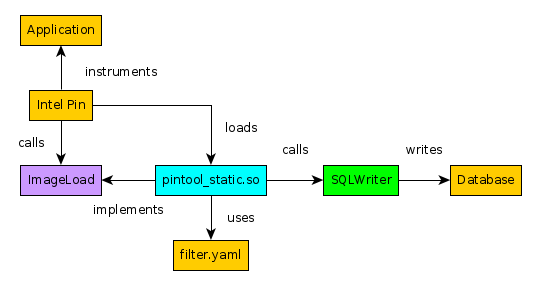
\includegraphics[width=1\textwidth]{static-arch}
	\caption{\texttt{pintool\_static.so} Architecture}
	\label{cap3:static-arch}
\end{figure}

\section{pintool\_dynamic.so}
\label{cap3:pintooldynamic}

\texttt{pintool\_dynamic.so} performs a dynamic analysis on the application.

\subsubsection{Architecture}

\begin{figure}
	\centering
	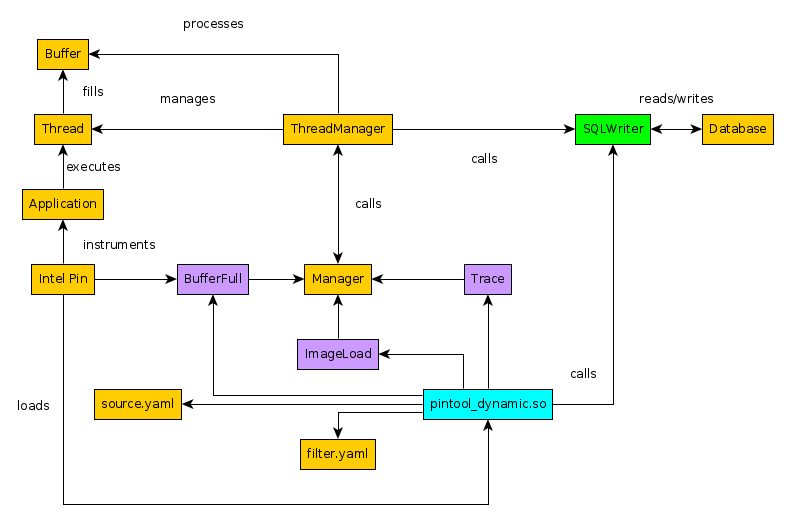
\includegraphics[width=1\textwidth]{dynamic-arch}
	\caption{\texttt{pintool\_dynamic.so} Architecture}
	\label{cap3:dynamic-arch}
\end{figure}

The architecture of \texttt{pintool\_dynamic.so} as can be seen in Figure \ref{cap3:dynamic-arch} is much more complex compared to the previous tool. Using the Fast buffer API has allowed us to cleanly separate the static analysis from the tracing that is performed.

The central component of this tool is the \texttt{Manager} class. It is a singleton that represents the state of the running program and is used to store information that is relevant for both analysis and tracing. Since calls to it are made from different threads calls to its methods and accesses to its members must be synchronized.

Each thread of the instrumented application is handled by a unique \texttt{ThreadManager}. It stores information relevant only to the specific thread and implements the buffer processing.

Static analysis is performed in the \texttt{ImageLoad} callback. Here the relationship between the \texttt{TagInstructions} and their corresponding instruction addresses is established. Inserting instrumentation at this point in time is not allowed by the Pin API and has been deferred to the \texttt{Trace} callback.

The \texttt{Trace} callback is called whenever new code is added to Intel Pins code cache \cite{pindoc}. Here we instrument the instructions that were marked by the static analysis.

The \texttt{SQLWriter} is part of the \texttt{Manager} singleton as only one connection to the database is active during the tracing. It is available to the static analysis and to all the \texttt{ThreadManager} instances. Synchronization of the connection is handled by the \texttt{SQLWriter} itself. 

\subsubsection{Fast buffer API}

The tool uses the Fast buffers API to reduce the overhead of the tracing. Currently only one buffer is used for the entire application and processing is not offloaded to a different thread to reduce complexity.

Many events are recorder in the buffer and the context of these events is recorded for later processing. The events handled by \texttt{pintool\_dynamic.so} are as follows:

\textbf{CallEnter} is recorded when the first instruction of a function is executed.

\textbf{Call} represents a call instruction. The next \textbf{CallEnter} determines to what function the call was made. 

\textbf{Ret} is a return instruction from a call.

\textbf{Tag} is recorded when a tagged instruction is encountered.

\textbf{MemRef} represents that a instruction has accessed one or more memory locations.

\textbf{AllocEnter} is recorded when the first instruction of a memory allocator function is executed.

\textbf{Free} is recorded when the first instruction of \texttt{free} executed.

\subsubsection{Shadow Call Stack}

Each \texttt{ThreadManager} contains a shadow call stack that is used when saving information about calls into the database, to determine the relationships between entities and to identify stack variables. Since the instruction stream of the application is filtered our shadow stack does not represent the complete stack of the managed thread, it only contains the functions that are interesting to the user.

Since the detection of return instructions is not always accurate \cite{pindoc} the shadow stack must sometimes be corrected to ensure a consistent state. This is achieved by recording the function that performed the return in the fast buffer, allowing all calls without a return instruction to be safely closed.

\subsubsection{Tagging implementation}

Determining whether a \texttt{TagInstruction} has been reached is simple using our implementation of tracing. During the static analysis the instructions that belong to lines that contain a \texttt{TagInstruction} are determined. During the \texttt{Trace} callback this inforation is used to insert instrumentation that records the execution of such an instruction.

The \texttt{ThreadManager} maintains a list of active \texttt{TagInstances} that is modified when a \texttt{TagInstruction} is encountered. This list is consulted for all the related events to save the relevant information into the database.

Custom logic is executed when a \texttt{TagInstances} starts and ends for each individual tag type. This allows tracing to be controlled using tags and analyses to be performed.

\subsubsection{Timing information}

\texttt{pintool\_dynamic.so} uses a processors built in high performance counter, the time stamp counter \cite{tsc}, to record timing information about many events. To ensure the correctness of this value all threads are bound to the processor core where they were first spawned.

Since the time stamp counter may advance at different speeds on independent processor cores, the values obtained by our tool need to be normalized. This is done by recording the unix time at the start and end of each threads and the amount of cycles executed by that thread. All events recorded in the database store a TSC value that is relative to the start of the thread.

During the database processing all TSC values are converted into a full date that was normalized for each thread independently.

\subsubsection{Memory allocation interception}

For both the user and the automated analyses it is important to be able to identify the type and lifetime of memory references. \texttt{pintool\_dynamic.so} identifies three types of references: stack variables, global memory and dynamically allocated references.

Stack variable information is maintained in the shadow call stack. Currently \texttt{pintool\_dynamic.so} ignores DWARF information related to memory references and stack variables are allocated when they are first used. Deallocaton is performed when a function returns.

Global variables are often used in programs and have the lifetime of the entire program. They are allocated on first use and are deallocated at the end of the execution.

Dynamically allocated memory requires the most complex handling. Calls to all memory allocation functions, \texttt{malloc}, \texttt{realloc} and \texttt{calloc}, and to \texttt{free} are intercepted to determine the lifetime of references. Due to the inability to find return instructions in these functions, routine instrumentation has been used.

The processing of buffers happens later than the routine instrumentation and the allocations detected by both processes must be correlated. This is done by storing the TSC of the function calls in both implementations and their relation can be easily established.

\subsubsection{Memory accesses}

All memory accesses made by unfiltered instructions are instrumented using the fast buffer API. This allows users and analyses to detect data and control dependencies in the application.

All accesses are instrumented, but only some are recorded in the database. This filtering is performed at run-time using tags as explained in Section \ref{controllingtracing}. This feature has been implemented due to the problems that Parceive \cite{parceive} has had with the large amounts of uninteresting accesses stored in the database.

\subsubsection{Reference resolution}

Recording only addresses for memory accesses in the database is insufficient for analyses and users alike. This information must be related to the known memory references of the instrumented application. Currently our tool does not parse DWARF information and only shows generated names for stack and global variables.

Each \texttt{ThreadManager} is able to determine the memory reference that contains a specific address. This resolution is done in multiple steps:

\begin{enumerate}
	\item If the address is part of a known memory reference, that reference is returned.
	\item Check whether the address is part of the stack of the current thread. If it is create a new stack reference and return it.
	\item If both previous steps failed create a new global memory reference and return it.
\end{enumerate}

All memory allocations (\texttt{malloc}, \texttt{calloc}, \texttt{realloc}) and deallocations (\texttt{free}) are instrumented in order to determine their lifetimes. The only way this can be done reliably on linux with Intel Pin is to replace the functions completely with a wrapper that calls the actual implementations and stores information about each call.

\section{Database writing}

\subsection{SQLite}

The SQLite library \cite{sqlitedoc} is used directly by both tools to read and write to a database. Unfortunately the locking mechanism used by the library can not be used directly as Intel Pin does not support using pthread locks. Because both tools use SQLite for a very specific purpose  we have decided to completely remove the locking implementation and to create a C++ wrapper around SQLite.

\subsection{SQLite Wrapper}

The primary purpose of the SQLite wrapper is to ensure correct synchronization of the underlying connection and statements. The locking is performed using Intel Pin mutexes.

The secondary purpose is to simplify the usage of the SQLite API. By using C++ and its RAII principle it is easier to manage connections and statements. Classes and templates provide OOP constructs that translate well to the native API.

Error handling is also completely handled by the wrapper. Our tools do not perform error recovery so all errors are handled as fatal and are logged appropriately. 

\subsection{SQLWriter Class}
\label{sqlwriter}

The \texttt{SQLWriter} class contains all prepared statements used by the tools and provides an API to insert and to query the tables. It is able to completely set up the database and to configure it for writing.

To increase writing speed SQLite has been configured in the following ways:

\begin{itemize}
	\item Journaling has been disabled.
	\item Foreign keys are not checked. The check is performed later during the database processing.
	\item Automatic vacuuming has been disabled. This process will be performed during the database processing.
	\item The database is opened in the exclusive mode. This denies access to other tools while working with the database.
\end{itemize}

Currently the \texttt{SQLWriter} class is focused almost completely on writing, reading being performed during the ImageLoad callback of \texttt{pintool\_dynamic.so}. The focus on writing allows the implementation to reduce the overhead of the tracing.

\section{Analysis}

\subsection{Calling Context Tree}

The CCT visualization can perform multiple basic analyses based on the information that is stored in the database. \texttt{pintool\_dynamic.so} is able to generate trace data required by them. The two most important ones are:

\subsubsection{Shared references}

Shared references analysis displays the shared references between multiple Calls, CallGroups, LoopExecutions and LoopIterations. This can be used to determine dependencies, but is very imprecise due to the fact that it does not consider any children of the processed entities.

\subsubsection{Shared recursive references}

Shared recursive references analysis improves upon the previous one by considering the entire call tree, but is limited to Calls and CallGroups.

\subsubsection{Issues}

\begin{enumerate}
	\item The execution time of both analyses increases sharply with the number of references used by the entire application.
	\item The detected dependencies can be false positives as the offset of the access within references is ignored. For example referencing different members of a structure will be falsely detected.
	\item The analysis is very coarse, working only with calls and loops.
\end{enumerate}

\subsection{Section}

\subsubsection{Introduction}

\texttt{pintool\_dynamic.so} can perform a fine grained detection of data and control dependencies that need to be addressed when parallelizing software. The user must tag sections and tasks within the code and the tool can automatically determine what tasks access a common reference.

\subsubsection{Parallelization}

This analysis assumes a very simple architecture. All tasks execute in parallel, but are all spawned and joined within a specific section. The order of execution between the tasks is not deterministic and as such all accesses to shared resources must be synchronized.

\subsubsection{Dependency detection}

The dependency detection is performed during the trace instrumentation as performing it later requires additional data to be stored in the database. The analysis also considers the lifetime of references in order not to create false positives when accessing stack variables that are local to the task.

Processing is performed during tracing and sequentially as each section is bound to a specific thread. First dependencies are determined as accesses to the same references, as is done by the CCT view. This ensures that the lifetimes of variables are taken into account. When a dependency is identified it is checked whether it has occurred on the same memory region to eliminate false positives. Lastly it is stored in the database for use by the visualization.

\subsubsection{Visualization}

The visualization for the section analysis renders two pieces of information that are relevant to the user. Firstly if shows the possible speedup when an ideal scheduling has een performed as can be seen in Figure \ref{cap3:sec:speedup} and the list of conflicts that need to be resolved in order to maintain correctness as can be seen in Figure \ref{cap3:sec:conflict}.

The simulation of parallel execution performs ideal scheduling of tasks on a configurable number of processing cores. The actual performance benefit is strictly lower that the value presented, but it can be used to check whether the parallelization is worthwhile. 

The list of conflicts is a simple table that lists all references that are accessed by different tasks. It integrates with the Detail view present in Parceive to shows where exactly the variable is accessed as can be seen in Figure \ref{cap3:sec:detail}.

\begin{figure}
	\centering
	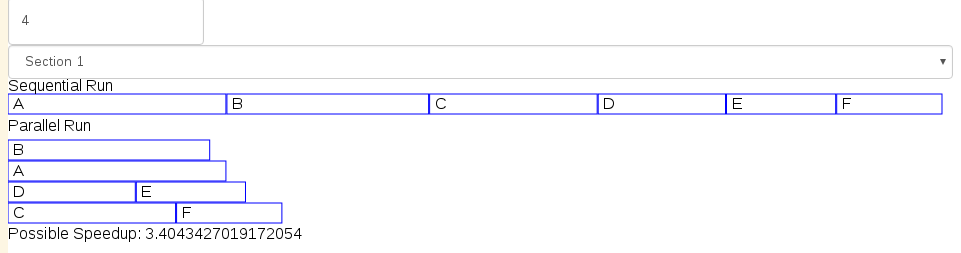
\includegraphics[width=1\textwidth]{section-speedup}
	\caption{Possible speedup}
	\label{cap3:sec:speedup}
\end{figure}

\begin{figure}
	\centering
	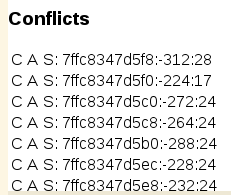
\includegraphics[width=0.4\textwidth]{section-conflict}
	\caption{Conflict list}
	\label{cap3:sec:conflict}
\end{figure}

\begin{figure}
	\centering
	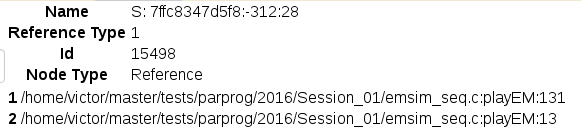
\includegraphics[width=1\textwidth]{section-detail}
	\caption{Access locations for a reference}
	\label{cap3:sec:detail}
\end{figure}

\subsection{Pipeline}
\subsubsection{Introduction}
\subsubsection{Parallelization}
\subsubsection{Dependency detection}
\subsubsection{Visualization}

\section{Visualizations}

Additional visualizations have been implemented to enable source code tagging and to display the information obtained by the analysis:

\textbf{File View}

The File View present in Parceive has been replaced with a more thorough solution. By using a different code highlighting tool \cite{googleprettify} it has become possible to refer to individual line in the source file. The new implementation allows the creation of TagInstructions on all lines that can be correlated to instructions in the application.

When working with a database that contains tracing information the visualization can be navigated more easily. Function definitions and calls are highlighted and can be focused in the source code view. This facilitates the edition of the tagging information for a new dynamic execution.

\textbf{Tag List}

\textbf{Section View}

\textbf{Pipeline View}

Additionally existing views have been extended to provide more information about tags:

\textbf{Detail View}

As can be seen in Figure \ref{cap3:detail} the detail view has been extended to show information about tags. 

\begin{figure}
	\centering
	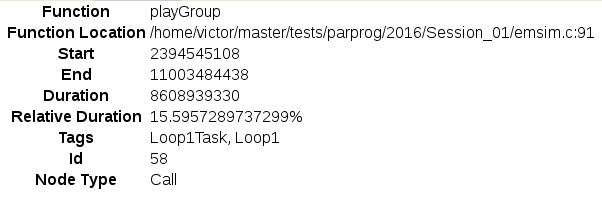
\includegraphics[width=1\textwidth]{detail-mod}
	\caption{Detail View modification}
	\label{cap3:detail}
\end{figure}

\textbf{CCT View}

The CCT View shown in Figure \ref{cap3:cct} has been extended to highlight the calls that have been made by tagged code. The Detail View can then be used to show the specific tags.

\begin{figure}
	\centering
	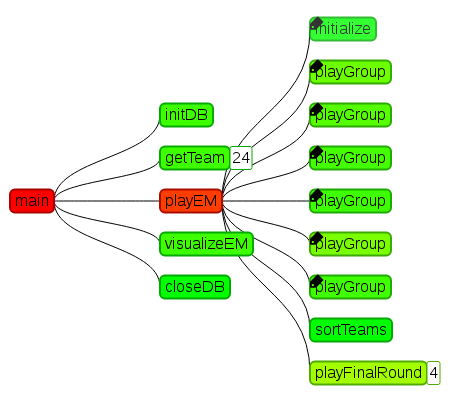
\includegraphics[width=1\textwidth]{cct-mod}
	\caption{CCT View modification}
	\label{cap3:cct}
\end{figure}






